%% Document created 20 March 2022 automatically 
%% from /Users/massimosotgia/Desktop/uni_at_DIFI/Lab2/setup.py 

%% Copyright (C) Mattia Sotgia et al. 2022
%% Using class revtex4-2.cls
%                                       
%                                       
%██       █████  ██████         ██████  
%██      ██   ██ ██   ██             ██ 
%██      ███████ ██████          █████  
%██      ██   ██ ██   ██        ██      
%███████ ██   ██ ██████  ██     ███████ 
%                                       
%                                       
\documentclass[
    rmp,
    % preprint,
    % linenumbers,
    % tightlines,
    reprint, 
    superscriptaddress, 
    altaffilletter, 
    amsmath, 
    amssymb, 
    a4paper, 
    fleqn]{revtex4-2}

\usepackage[top=1.75cm,bottom=2.5cm,left=1.5cm,right=1.5cm]{geometry}

\usepackage[utf8]{inputenc}
\usepackage[T1]{fontenc}

\usepackage[italian]{babel}

%% revtex4-2 bug-fix
\def\andname{e}
%--------------------
\makeatletter
\let\it@comma@def\active@comma
\makeatother

\usepackage{txfonts}
\usepackage{graphicx}% Include figure files
\graphicspath{{../fig/}}

\usepackage{dcolumn}% Align table columns on decimal point
\usepackage{bm}% bold math
\usepackage[colorlinks, urlcolor=., bookmarks]{hyperref}% add hypertext capabilities
\renewcommand\UrlFont{\color{blue}}

\usepackage{physics}
\usepackage{siunitx}

\usepackage{fancyhdr}
\pagestyle{fancy}
\fancyhf{}
\def\twodigits#1{\ifnum#1<10 0\fi\the#1}

%-----------------------------------------------------------------------------------------------

\usepackage{background}
\SetBgColor{gray}
\SetBgAngle{90}
\SetBgScale{2}
\SetBgVshift{0.27\textwidth}

\usepackage[american resistors]{circuitikz}
\usepackage{listings}
\lstset{
  basicstyle=\fontsize{5}{6}\selectfont\ttfamily,
  % backgroundcolor=\color{white},   % choose the background color
  % basicstyle=\footnotesize,        % the size of the fonts that are used for the code
  breakatwhitespace=false,         % sets if automatic breaks should only happen at whitespace
  breaklines=true,                 % sets automatic line breaking
  captionpos=b,                    % sets the caption-position to bottom
  % commentstyle=\color{mygreen},    % comment style
  deletekeywords={...},            % if you want to delete keywords from the given language
  escapeinside={\%*}{*)},          % if you want to add LaTeX within your code
  % extendedchars=true,              % lets you use non-ASCII characters; for 8-bits encodings only, does not work with UTF-8
  % firstnumber=1000,                % start line enumeration with line 1000
  % frame=single,                    % adds a frame around the code
  % keepspaces=true,                 % keeps spaces in text, useful for keeping indentation of code (possibly needs columns=flexible). 
  % keywordstyle=\color{blue},       % keyword style
  % numbers=left,                    % where to put the line-numbers; possible values are (none, left, right)
  % numbersep=5pt,                   % how far the line-numbers are from the code
  numberstyle=\tiny\color{gray}, % the style that is used for the line-numbers
  % rulecolor=\color{black},         % if not set, the frame-color may be changed on line-breaks within not-black text (e.g. comments (green here))
  showspaces=false,                % show spaces everywhere adding particular underscores; it overrides 'showstringspaces'
  showstringspaces=false,          % underline spaces within strings only
  showtabs=false,                  % show tabs within strings adding particular underscores
  stepnumber=2,                    % the step between two line-numbers. If it's 1, each line will be numbered
  % stringstyle=\color{mymauve},     % string literal style
  tabsize=2,                       % sets default tabsize to 2 spaces
}
\usepackage{soul}


%% Define ref types
\newcommand{\reftab}[1]{Tabella {\ref{#1}}}%
\newcommand{\reffig}[1]{Figura {\ref{#1}}}%
\newcommand{\refeqn}[1]{({\ref{#1}})}%
\newcommand{\ChiSqr}{$\chi^2$\space}
\newcommand{\ChiNdf}{$\chi^2/\text{ndf}$}
\newcommand{\cernroot}{\texttt{root}}
\newcommand{\treSigma}{$3\sigma$}
\newcommand{\stdErr}[1]{$\varepsilon_{#1}$}
\newcommand{\mstdErr}[1]{\varepsilon_{#1}}
%% PAPER ONLY custom Macros

\newenvironment{methods}[1]{\section*{#1}
%\fontfamily{phv}
\fontsize{7.5}{9}\selectfont\label{sec:methods}\noindent}{\par\noindent}

%\usepackage{lcsec}


\fancyfoot[C]{
    \the\year\twodigits\month\twodigits\day/6-\thepage
}
\fancyhead[C]{\fontfamily{phv}\fontsize{12}{12}\selectfont RELAZIONE DI LABORATORIO \textbf{
    N. 3 % ! <== CAMBIARE (Nessuna rel. -> 00)
    } (\the\year)
}

\begin{document}

\title{Misura della velocità del suono in aria
}
\thanks{Esperienza n. 6
}

\author{Francesco Polleri}
\email{s5025011@studenti.unige.it}
\author{Mattia Sotgia}
\email{s4942225@studenti.unige.it}

\collaboration{Gruppo A1}
\affiliation{Dipartimento di Fisica, Università degli Studi di Genova, I-16146 Genova, Italia}

\date{presa dati
    20 marzo 2022, consegnata in data 
    \today
}

\begin{abstract}

\end{abstract}

\maketitle
\thispagestyle{fancy}
% Rimuovere per consegna
\SetBgContents{
    laboratorio2: e6 [non per la consegna] \today % ! Note di versione
}


%%%% CORPO DEL TESTO
%%%% CORPO DEL TESTO


\section{Introduzione}

L'obiettivo di questa esperienza di laboratorio è effettuare una misura della velocità del suono in aria. Per ottenere tale misura sfruttiamo l'intervallo di tempo che l'onda sonora impiega a percorrere la distanza che separa l'emettitore e il ricevitore. Infatti, una volta misurato tale intervallo di tempo, è necessario solamente conoscere appunto la distanza tra i due dispositivi per ricavare la velocità del suono. Il problema principale è però ottenere una misura precisa del tempo in quanto sappiamo che l'intervalli che andiamo a misurare sono molto brevi perchè il suono viaggia ad una velocità di circa \SI{340}{\metre\per\second} per cui se posizioniamo emettitore e ricevitore ad una distanza nell'ordine delle decine di centimetri il tempo che l'onda impiega a percorrere tale distanza sarà allora nell'ordine dei millisecondi. 
Per misurare gli intervalli di tempo utilizziamo quindi due diversi metodi. Il primo metodo consiste nell'effettuare la misurazione in maniera analogica, osservando sull'oscilloscopio il ritardo temporale che intercorre tra il segnale prodotto dall'emettitore e il segnale prodotto dal ricevitore. Il secondo metodo invece ??? 

\section{Caratterizzazione apparato sperimentale analogico}

Il sistema di misura è composto da un emettitore ed un ricevitore posti ad una distanza $d=[0.1, 0.5]~\si{\metre}$. Questi due strumenti messi in comunicazione con un oscillatore ci permettono di misurare il ritardo tra il fronte dell'onda trasmessa e quello dell'onda ricevuta, permettendoci di individuare il ritardo tra le due onde, e quindi inferire il valore della velocità del suono in aria. 

\paragraph*{L'emettitore} L'emettitore consiste in un semplice altoparlante elettronico (attuatore), caratterizzato da un diametro esterno di \SI{5.985+-0.005}{\centi\metre} capace di convertire in onde sonore un segnale che può essere fornito in ingresso. Questo viene alimentato dal generatore digilab che permette di fornire in ingresso un'onda quadra, di frequenza e ampiezza variabile. Il generatore digilab fornisce inoltre anche un segnale TTL standardizzato che può essere utilizzato come riferimento per la misura di quest'onda. Per la misura si è utilizzata un'onda quadra di frequenza variabile (in base alle necessità della misura) tra \SI{10}{\hertz} e \SI{10}{\kilo\hertz}.

\paragraph*{Il ricevitore} Lo strumento è composto da un microfono (trasduttore) che permette di convertire in segnale analogico l'onda sonora che riceve. Il segnale analogico continuo viene poi mandato in ingresso ad un comparatore a soglia fissa, che quindi permette di ottenere solo due letture in uscita, un segnale alto e un segnale basso. 


\begin{figure}[b]
    \centering
    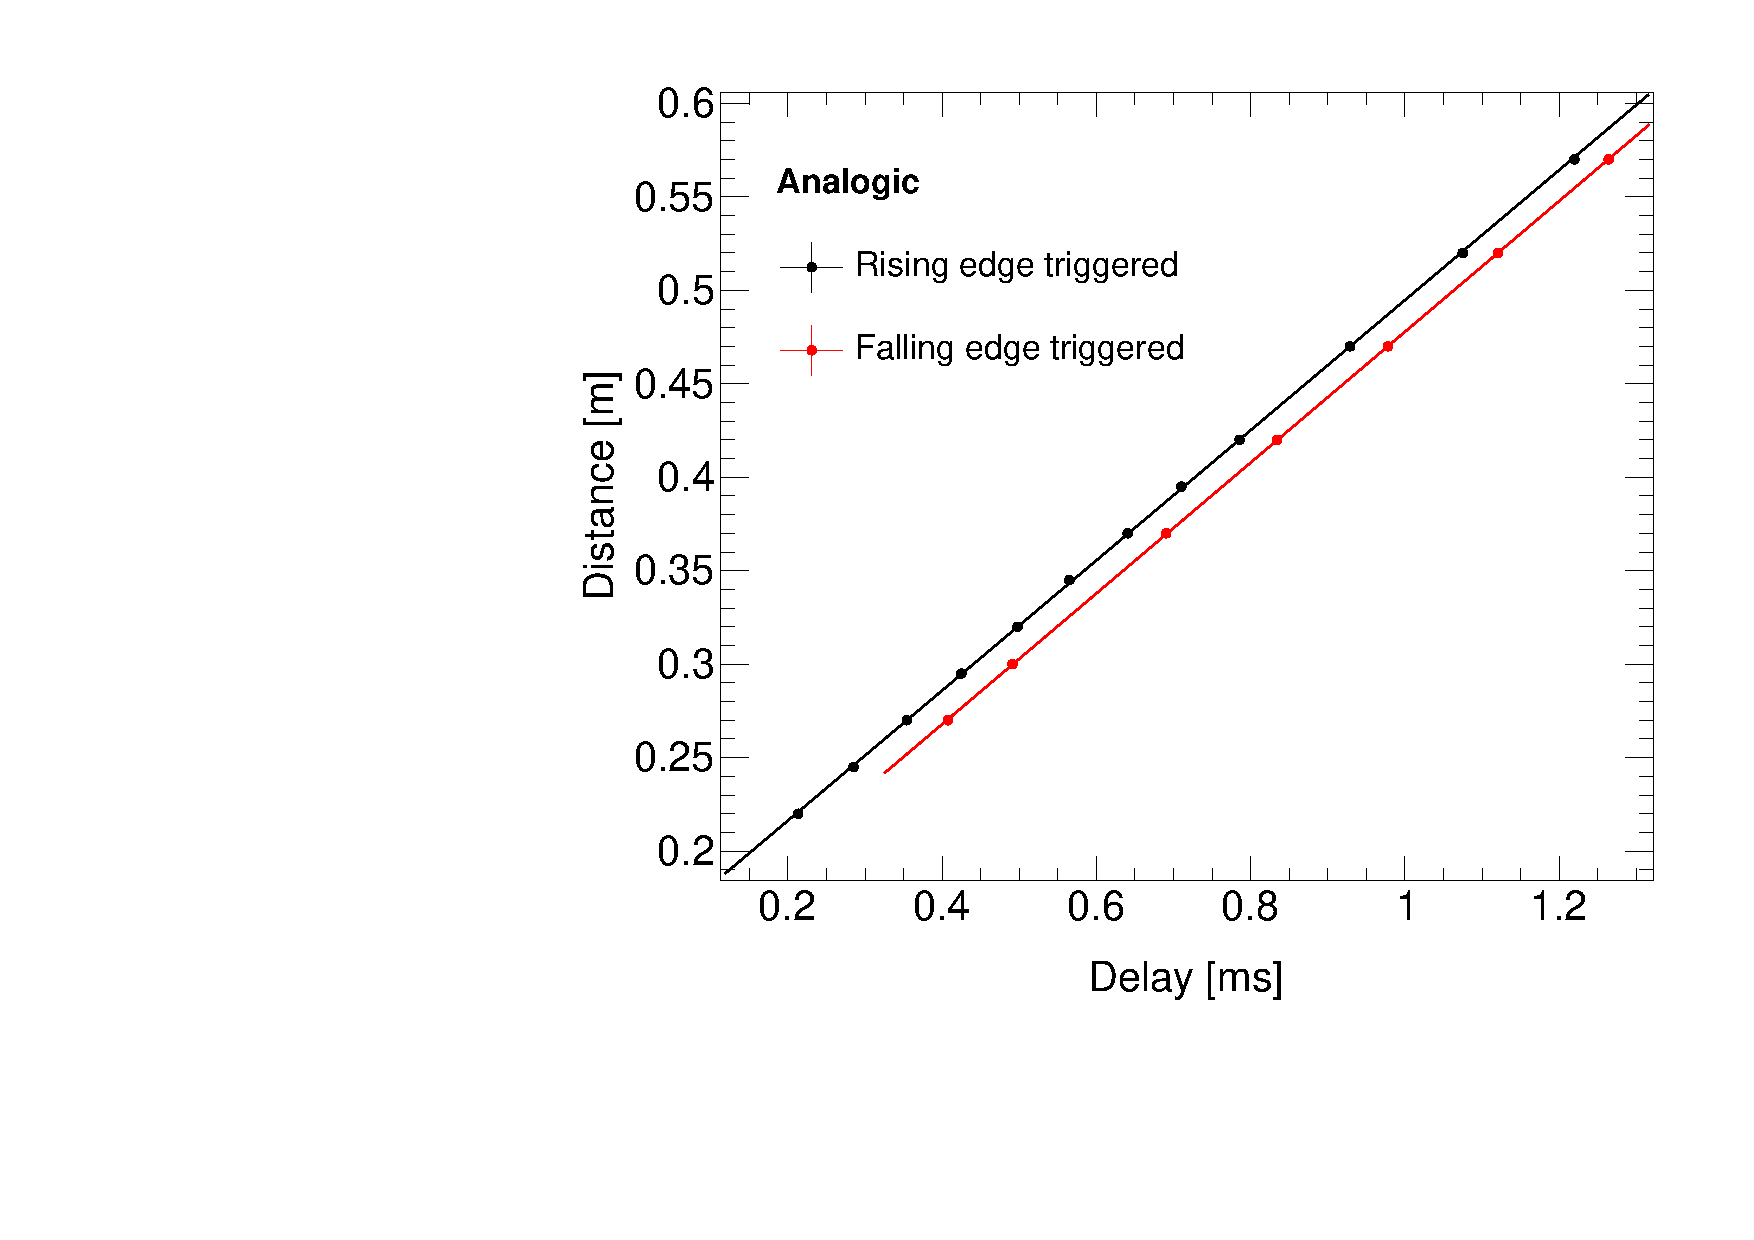
\includegraphics[width=0.75\linewidth]{analog_plot_a220402.pdf}
    \caption{Dipendenza lineare del ritardo dal tempo $t$, il coefficiente di proporzionalità esprime la velocità di propagazione di un onda sonora in aria.}\label{fig:analog_plot_d1}
\end{figure}


\section{Conclusioni}


%\onecolumngrid
\appendix

\setcounter{table}{0}
\renewcommand{\thetable}{A-\Roman{table}}

\end{document}
    
